\documentclass[12pt]{article}
\usepackage[spanish]{babel}
\usepackage[utf8]{inputenc}
\usepackage{graphicx}
\title{Disciplina de Requisitos}
\date{2025-06-02}
\usepackage[margin=1in]{geometry}
\begin{document}
    \begin{titlepage}
        \centering
        {\Large Universidad Central de Venezuela \par}
        \vspace{0.25cm}
        {\Large Facultad de Ciencias \par}
        \vfill
        {\LARGE Proyecto: Comedor Universitario \par}
        \vspace{0.25cm}
        {\bfseries\Huge Disciplina de Requisitos \par}
        \vfill
        \raggedright
        {\large Profesor: Marcel Castro \par}
        {\large Sección: C2 \par}
        \vspace{0.5cm}
        {\large Equipo \#4: \par}
        \begin{itemize}
            \item {\large Samantha Arellano} - C.I.30.830.771
            \item {\large Tobias Briceño} - C.I. 31.307.238
            \item {\large María Laura Reina} - C.I. 31.275.108
            \item {\large Victoria Ruza} - C.I. 30.946.460
        \end{itemize}
        \vspace{1cm}
        \centering
        {\large 2 de junio del 2025 \par}
    \end{titlepage}

    \section{Visión del producto}
    
    \begin{table}[t]
        \begin{center}
        \begin{tabular}{| c | c | c | c | }
        \hline
        \multicolumn{2}{ |c| }{A}{B}\\ \hline
        Fabricante & Modelo & Clase & Motor \\ \hline
        BMW & Serie 3 & Berlina & Diésel \\
        Peugeot & 508 & Berlina & Gasolina \\
        Chrysler & Voyager & Monovolumen & Gasolina \\
        Land Rover & Defender & Todoterreno & Gasolina \\ \hline
        \end{tabular}
        \label{tab:coches}
        \end{center}
    \end{table}

    \section{Diagrama de casos de uso}
    \begin{center}
        \vfill
        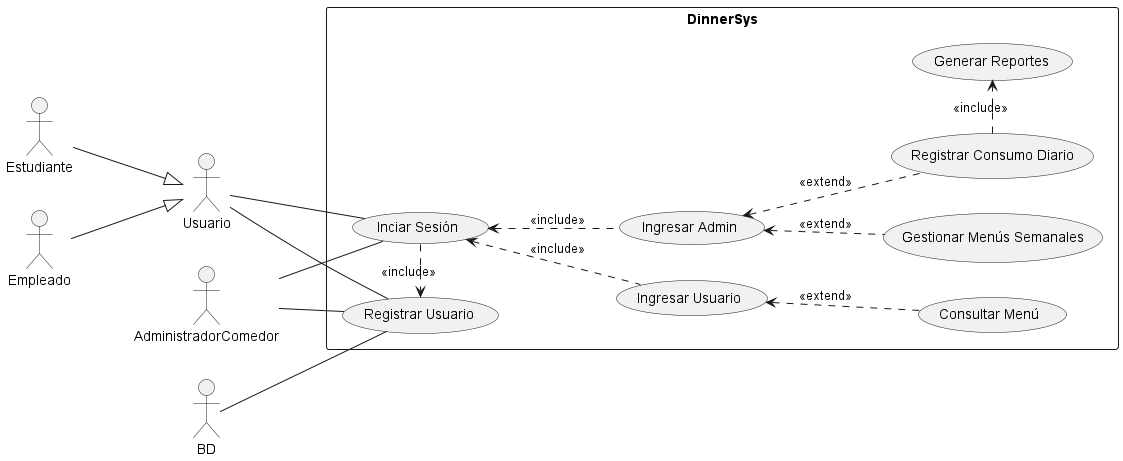
\includegraphics[width=10cm]{Partes/casosDeUso.png}
        \vfill
    \end{center}
\end {document}